The Brew System layer is the core of the Back Burner Brew. The goal of the project is to automate the brewing process, and although the system itself is very simple, the steps required to brew a proper beer is time consuming and requires a large amount of attention from the brewer. The user interface layer will ask the brewer to enter their desired temperature and time for each step of the brewing process. The analog and digital components will send data to the digital components. This data will contain the temperatures of the Hot Liqour Tank (HLT) and the mash tun, once the data is receieved by the digital components, the Web server layer will store that data into a cloud database and that data will be used to determine when a heating element or pump will turn on.
\begin{figure}[H]
	\centering
	\graphicspath{.\images}
	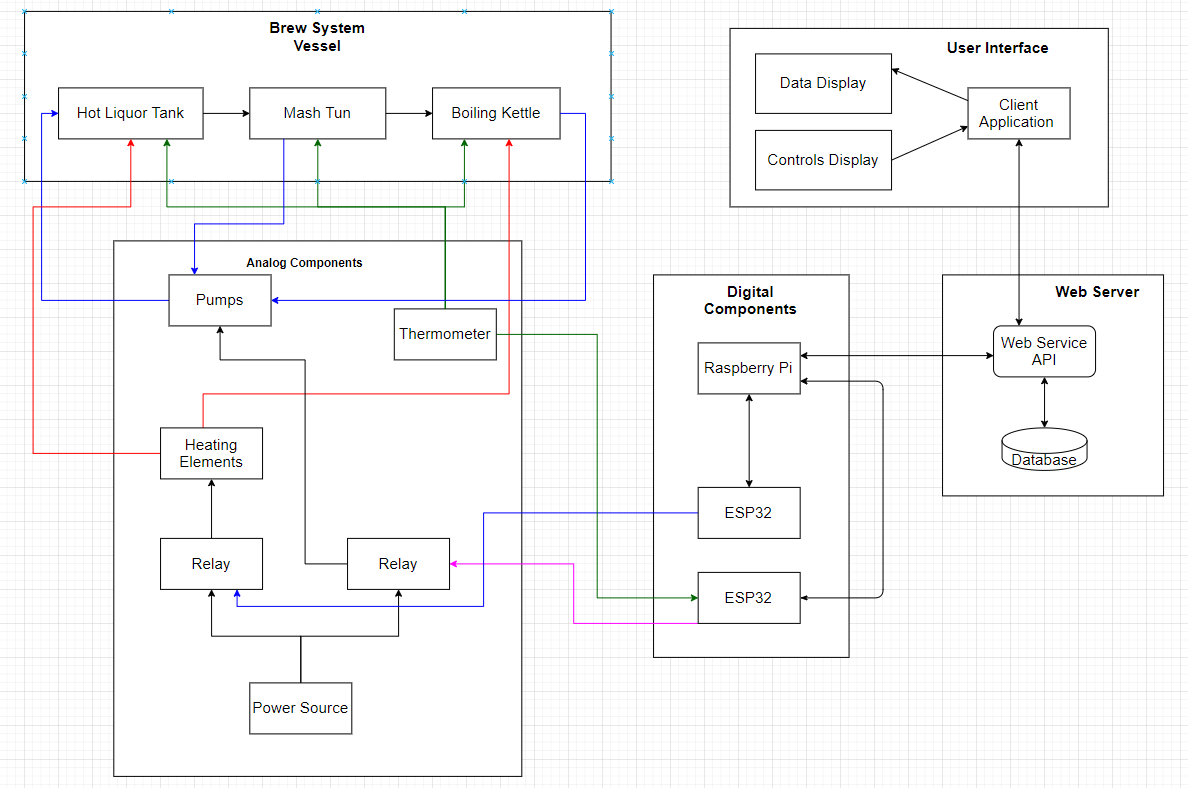
\includegraphics[scale=0.5]{images/sys_overview.PNG}
	\caption{System Overview}
\end{figure}